\chapter{Communication Protocol}
\label{cha:comm-prot}

\section{Network Topology}
\label{sec:network-topology}

\begin{figure}
  \begin{center}
    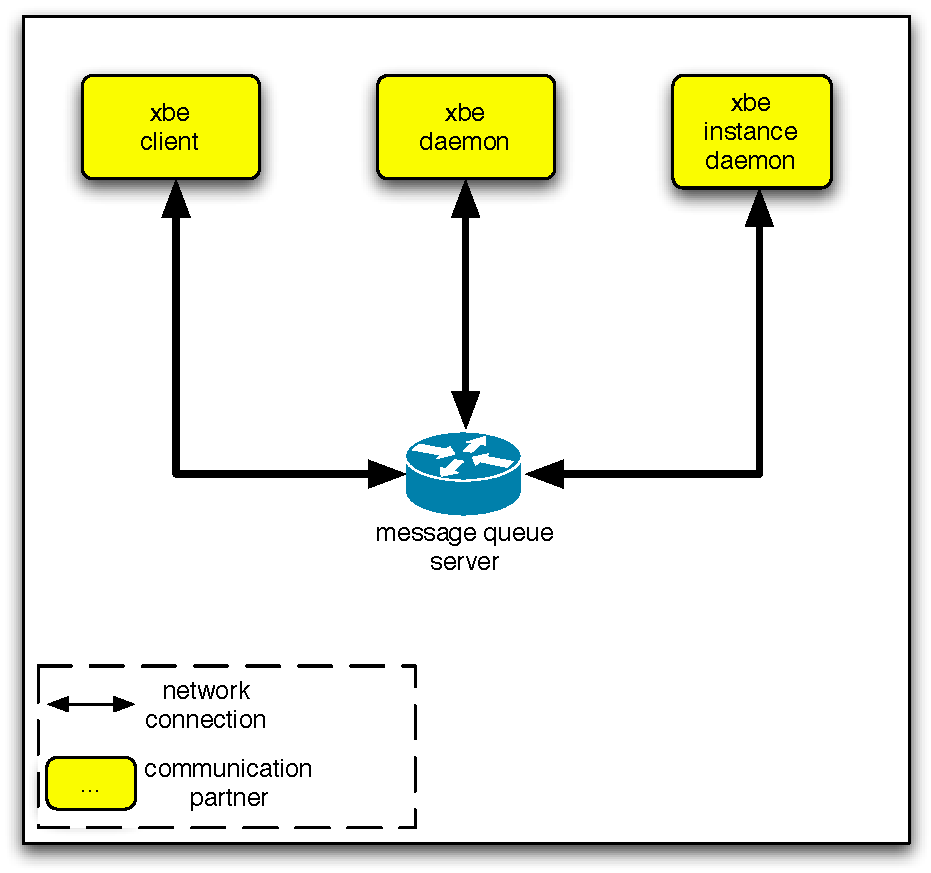
\includegraphics[scale=.75]{simple-network-topology}
  \end{center}
  \caption[Network  Topology   (simple)]{The  simplest  network  topology,
    consisting of  only one Message  Queue Server and  three communication
    partners.}
  \label{fig:simple-net-top}
\end{figure}

\begin{figure}
  \begin{center}
    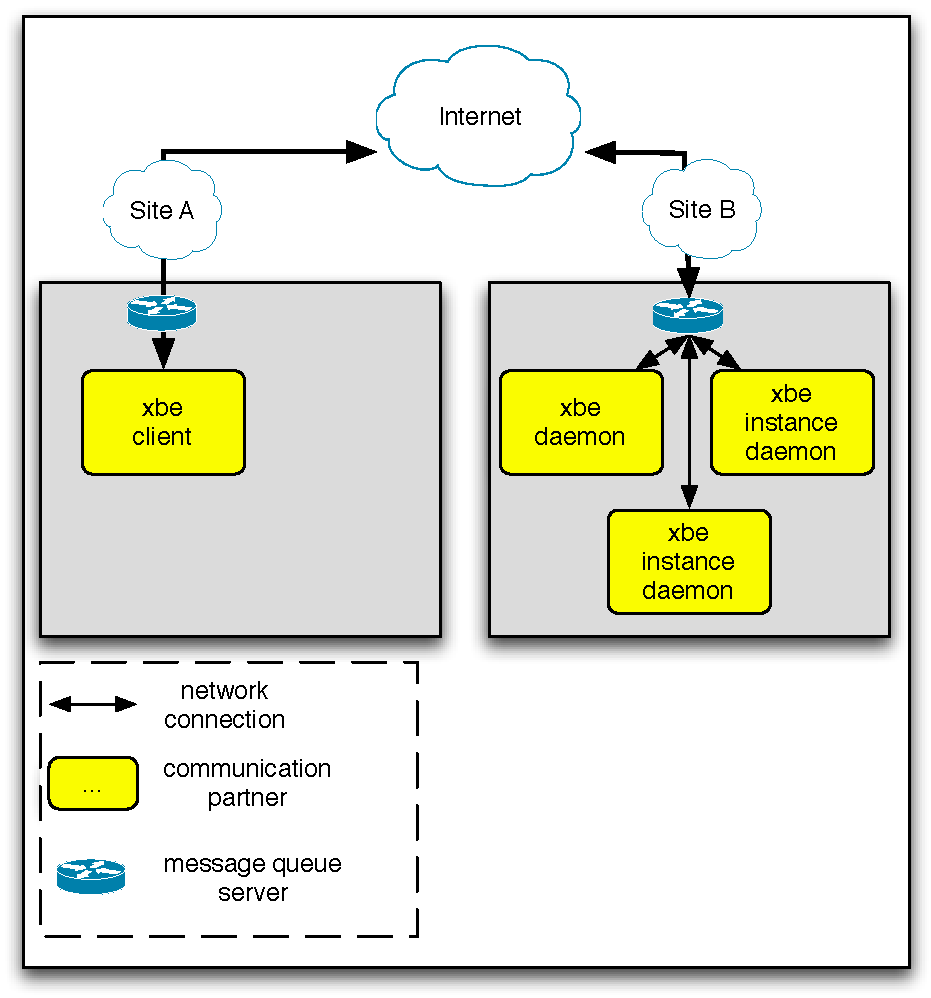
\includegraphics[scale=.75]{network-topology}
  \end{center}
  \caption[Network  Topology]{TODO: fill me in}
  \label{fig:net-top}
\end{figure}

\begin{figure}
  \begin{center}
    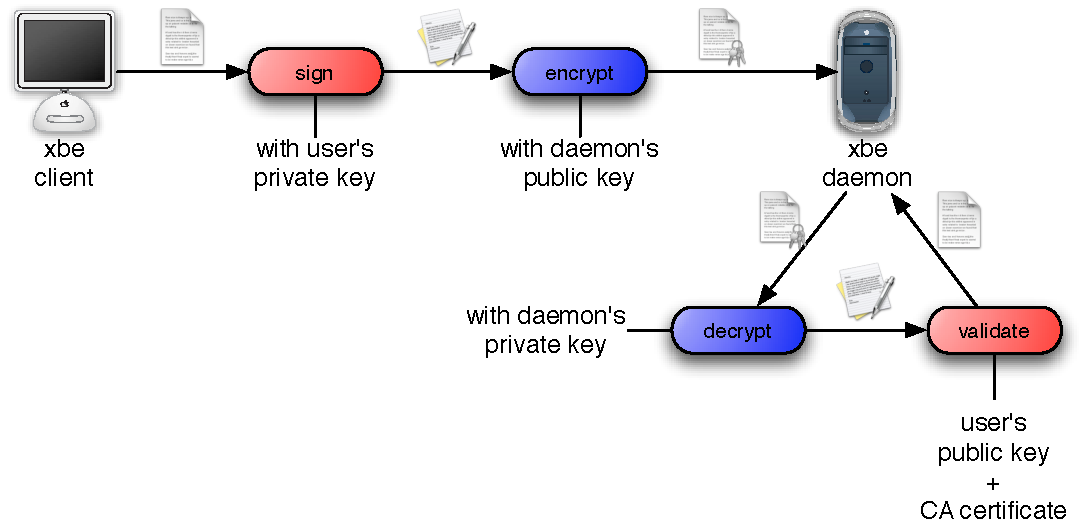
\includegraphics[scale=.75]{message-layer-security}
  \end{center}
  \caption[Message Layer Security]{TODO: fill me in}
  \label{fig:net-mls}
\end{figure}

\begin{figure}
  \begin{center}
    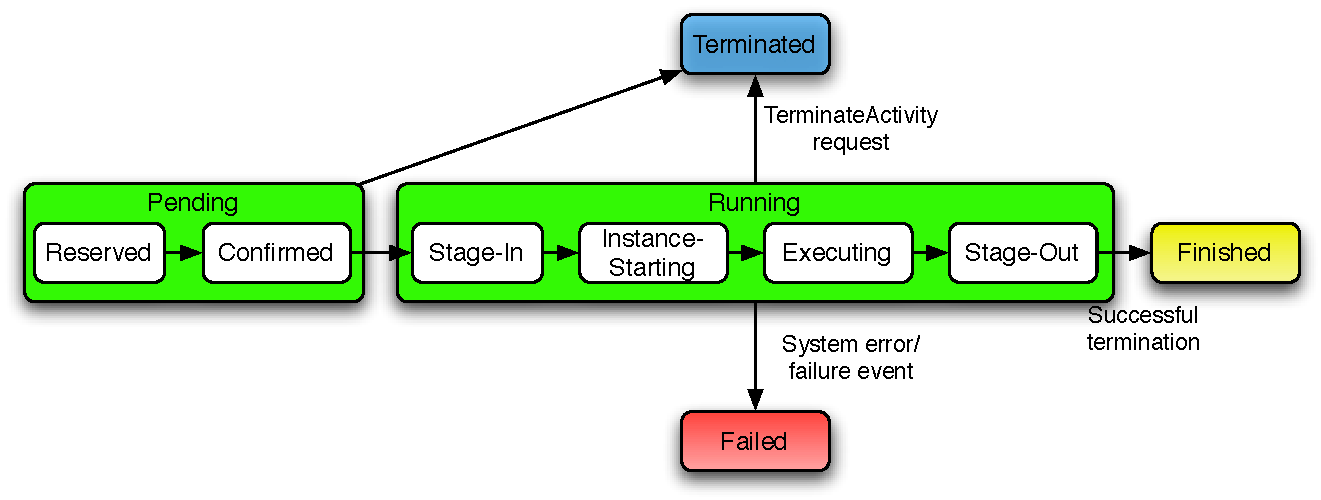
\includegraphics[scale=.75]{extended-job-model}
  \end{center}
  \caption[Job Model (extended)]{TODO: fill me in}
  \label{fig:bes-extended-xen}
\end{figure}

%%% Local Variables: 
%%% mode: latex
%%% TeX-master: "main"
%%% End: 
